
\chapter{Photocyclization Dynamics of Diarylethene}
\label{ch: UED-DAE}

The focus of this chapter is a study that uses UED to probe the atomic motions
that take place during the `photocyclization' or
photoinduced ring-closing reaction of the molecule
1,2-bis(2,4-dimethyl-5-phenyl-3-thienyl)perfluorocyclopentene,
herein abbreviated to PFC.
%
I will give an overview on the properties and photophysics of the family of molecules
known as `diarylethene,' to which PFC belongs.
%
Then, I will describe the experimental methods involved and
finally discuss the results from the measurements. Large portions of this chapter
is based on the work described in the article ``Ring-Closing Reaction in Diarylethene
Captured by Femtosecond Electron Crystallography'' previously published in
the Journal of Physical Chemistry~B~\cite{Jean-Ruel2013}.

\section{Overview of Diarylethenes}
\label{sec: UED-DAE-Intro}

A diarylethene is a pair of double-bonded carbon atoms with an aryl%
\footnote{An aryl is any molecular substituent derived from an aromatic ring,
e.g.~phenyl (C\textsubscript{6}H\textsubscript{5}--) is
the aryl of benzene (C\textsubscript{6}H\textsubscript{6}).} group attached to each end;
%
Its chemical derivatives form a distinct family of molecules that exhibit `photochromism' or
light-induced reversible colour change by chemically transforming between isomers
with different absorption spectra.
%
As seen in Fig.~\ref{fig: DAE-overview}, they go from colourless to coloured and
the absorption of the photogenerated state can be tuned across the visible spectrum
with appropriate modification of the base molecular structure.
%
In particular, DAEs are `P-type' photochromes;
their coloured forms are thermodynamically stable and can only be converted back photochemically.
Others photochromes, like azobenzenes and spiropyrans, have thermally driven back-reactions
and are thus known as `T-type.'
%
This means that the photochromic state of P-type DAEs is non-volatile and
can be addressed and changed using light only, properties that make such molecules
prime candidates for use in optoelectronics, such as optical memory devices and photoswitches,
and in optomechanics, as light-driven actuators and molecular machines~\cite{Irie2000, Irie2014}.

\begin{figure}[t!]
  \centering
  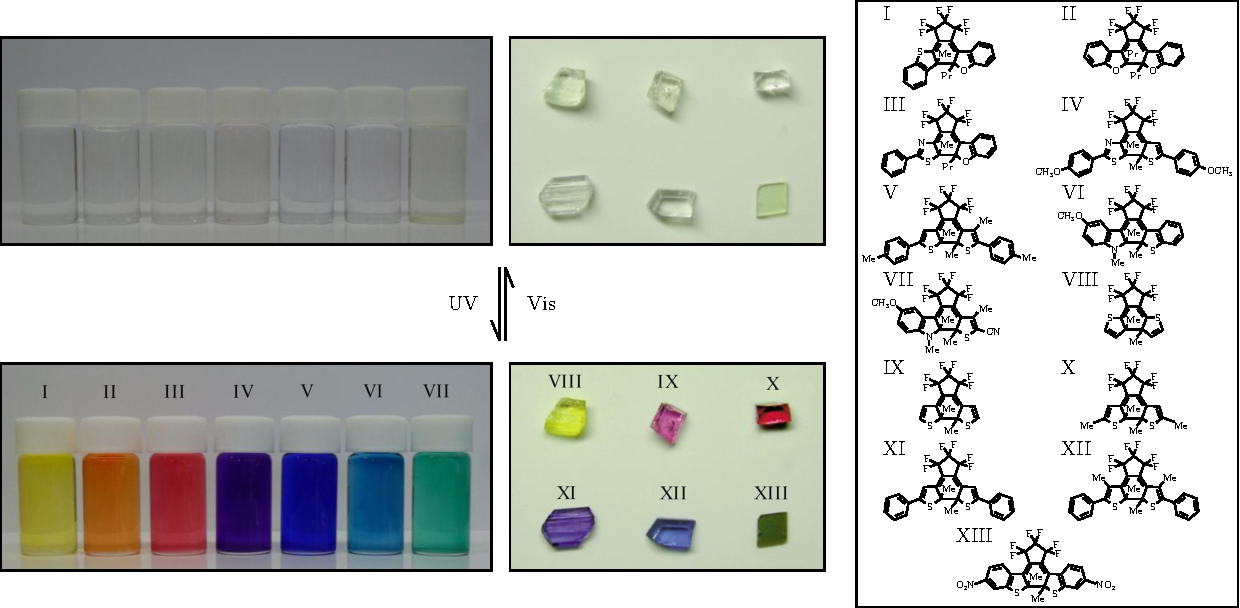
\includegraphics[width = \textwidth]{Figures/fig_DAE_overview.pdf}
  \caption[Photochromism of diarylethene derivatives.]{
    Photochromism of diarylethene derivatives in toluene~(left) and
    in single crystal~(centre) under $266$-nm light;
    their molecular structures are shown on the right.
    Adapted with permission from Ref.~\cite{Irie2014}.
  }
  \label{fig: DAE-overview}
\end{figure}

A prototypical diarylethene is 1,2-diphenylethene or stilbene~(\textbf{1});
As shown in Fig.~\ref{fig: DAE-stilbene}, its colourless \textit{cis}%
\footnote{The prefixes \textit{cis} and \textit{trans} denote the side on which
a pair of functional groups is relative to a carbon chain:
\textit{cis} = same side; \textit{trans} = opposite sides.}
or open-ring~(OR) form can reversibly photoisomerize under UV radiation to
the \textit{trans} form~(\textbf{2})
or undergo `photocyclization'~(ring-closing) and become yellow 4a,4b-dihydrophenanthrene~(\textbf{3}).
In the absence of oxygen, this coloured closed-ring~(CR) conformer
quickly reverts back to \textbf{1} in the dark via `cycloreversion'~(ring-opening);
otherwise, it oxidizes irreversibly to phenanthrene~\cite{Bao2011}.
%
\begin{figure}[ht!]
  \centering
  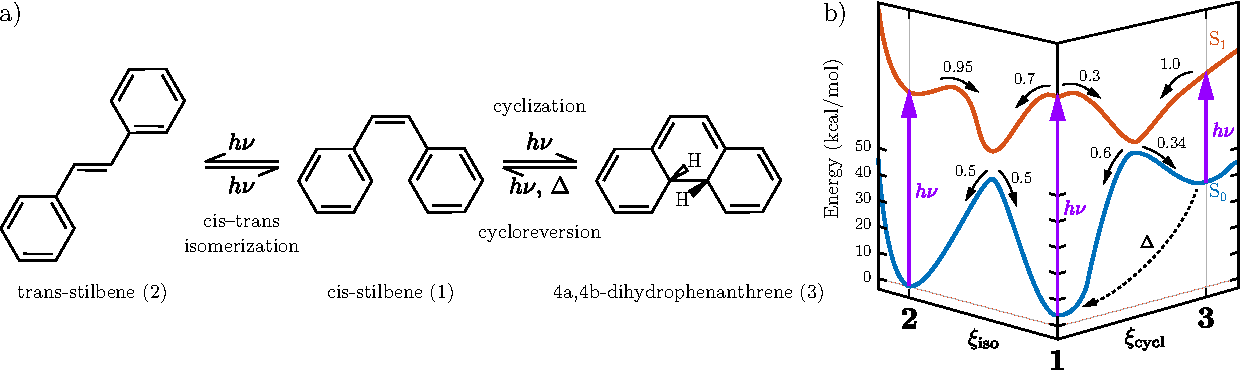
\includegraphics[width = \textwidth]{Figures/fig_DAE_stilbene.pdf}
  \caption[Photochemical reactions of \textit{cis}-stilbene.]{
    Photochemical reactions of \textit{cis}-stilbene.
    (a) Under UV exposure, \textit{cis}--\textit{trans} isomerization,
    cyclization, and cycloreversion can occur.
    (b) Schematic of the potential energy surfaces of the S$_1$ photochemical processes
    of stilbene along the two reaction coordinates;
    approximate quantum yields and branching ratios are indicated.
    Adapted with permission from Ref.~\cite{Repinec1991}.
  }
  \label{fig: DAE-stilbene}
\end{figure}

As noted in Ref.~\cite{Irie2014},
a DAE molecule optimized for the practical applications laid out earlier ought to satisfy
the following requirements:
%
\begin{enumerate}
  \item thermal stability of both colourless and coloured isomers;
  \item resistance to fatigue over multiple photocycles;
  \item high quantum yield;
  \item ultrafast response;
  \item activity in solid state;
  \item sensitivity in the near-IR region (650--830~nm).
\end{enumerate}
%
Clearly, \textit{cis}-stilbene is inadequate and a great number of derivatives
have been chemically synthesized to remediate its lackluster photochromic properties~\cite{Szaloki2013}.
One substitution pathway is as follows.
To prevent thermal cycloreversion of \textbf{1}, the phenyl groups are replaced by
thiophene rings which reduce the aromaticity, and thus the ground state energy,
of the coloured CR isomer~\cite{Irie1988, Irie1989}.
%
To stabilize the ring-closed isomer against oxidation and optical fatigue,
methyl groups are substituted at both \textit{ortho}-positions
of the thiophene--ethene bond~\cite{Irie1999, Higashiguchi2000};
%
To increase the quantum yield of the photochromic cyclization,
the \textit{cis}--\textit{trans} photoisomerization is blocked
by replacing the ethene moiety with a cyclopentene ring;
fluorination of this ring speeds up the ring closure (from $4.2$ to $0.9$~ps)~\cite{Hania2005}.
%
Substitution of a phenyl ring onto each thiophene ring increases
the peak absorption coefficient~$\epsilon$ of the CR isomer
(from $5.0 \times 10^3$ to $1.1 \times 10^4$~M$^{-1}$~cm$^{-1}$)
and shifts its absorption maximum a bit closer to the near-IR (from $534$ to $560$~nm%
\footnote{In benzene.})~\cite{Irie2014}.
The result is a diarylethene derivative called
1,2-bis(2,4-dimethyl-5-phenyl-3-thienyl) perfluorocyclopentene~(PFC)
and its molecular structure is shown in Fig.~\ref{fig: DAE-PFC}a.

\begin{figure}[t!]
  \centering
  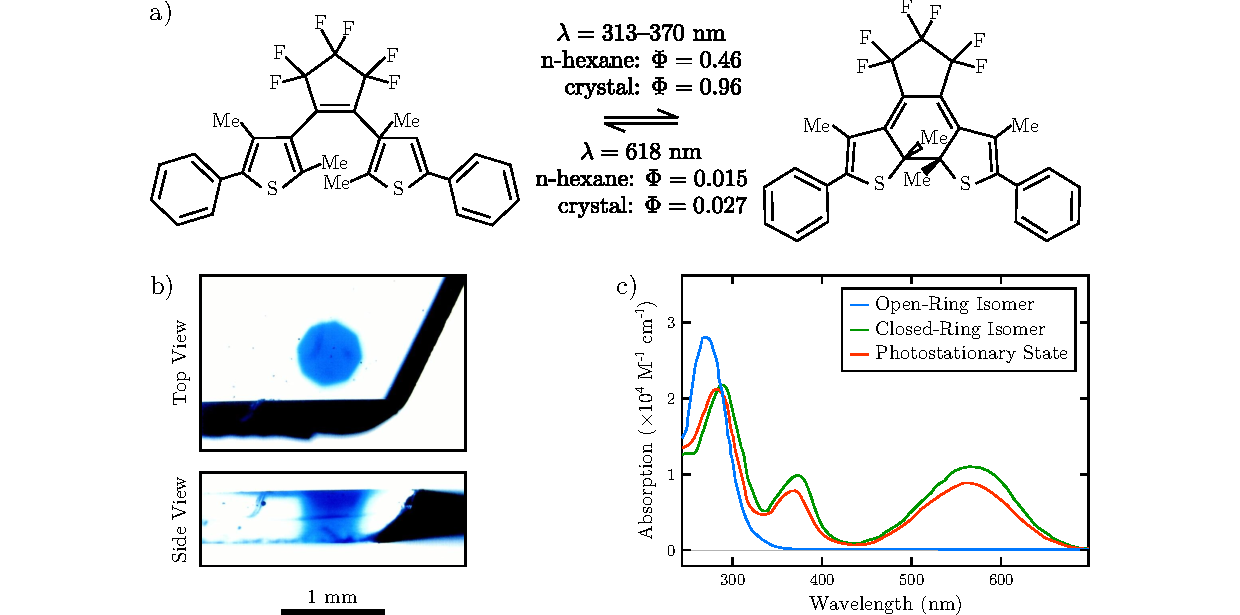
\includegraphics[width = \textwidth]{Figures/fig_DAE_PFC.pdf}
  \caption[Overview of 1,2-bis(2,4-dimethyl-5-phenyl-3-thienyl)perfluorocyclopentene.]{
    Overview of photochromism in PFC:
    (a) molecular structure,
    (b) photochromism in single-crystal (top and side view, circular spot under 366-nm light), and
    (c) absorption spectrum in n-hexane of the open-ring and closed-ring conformations;
    The values for the quantum yield $\Phi$ of the ring-closing/opening reactions
    in n-hexane and in single-crystal in Panel~(a) are taken from
    Refs.~\cite{Irie1995, Shibata2002} respectively.
    Panels~(b) and (c) are adapted with permission
    from Refs.~\cite{Irie2001} and~\cite{Irie1995} respectively.
  }
  \label{fig: DAE-PFC}
\end{figure}

PFC is a DAE molecule that has been often studied
since it is first reported by Irie et al~\cite{Irie1995}.
%
As seen in Fig.~\ref{fig: DAE-PFC}c,
the OR isomer of this molecular system is transparent to visible light,
absorbing strongly in the UV part of the spectrum%
\footnote{Absorption of PFC in n-hexane: $\lambda_\mathrm{max} = 268$~nm (OR) and $562$~nm (CR),
$\epsilon = 2.84 \times 10^4$~M$^{-1}$~cm$^{-1}$ (OR)
and $1.09 \times 10^4$~M$^{-1}$~cm$^{-1}$ (CR)~\cite{Irie1995}.}
to drive photocyclization to the CR conformation which appears blue (Fig.~\ref{fig: DAE-PFC}b).
%
In single crystal, this change in molecular structure is sufficiently large
to create regular $1$-nm tall steps and ridges on the material surface
that disappear upon cycloreversion~\cite{Irie2001}.
%
Furthermore, the quantum yield of the ring-closing reaction in this state
is more than double that in the solution phase
since all the thiophene side-groups of the OR isomers are locked in an anti-parallel conformation
wherein the reactive carbon atoms are in close proximity~\cite{Shibata2002};
in solution, the substituents are free to rotate and $52$~\% of them are aligned in parallel,
causing the molecule to be nonreactive to photocyclization~\cite{Irie1995, Pontecorvo2014}.

A large number of works has studied the electronic reaction dynamics of
photo-cyclization and -cycloreversion of DAE derivatives in the solution phase
using time-resolved spectroscopic techniques;
indeed, the processes were found to be ultrafast,
having taken place within a few picoseconds~\cite{Irie2014}.
%
More relevant to UED are some studies which were made on PFC and its close relatives
in the crystalline phase~\cite{Miyasaka1997, Ishibashi2007, Tani2008, Jean-Ruel2011}.
%
In particular, Jean~Ruel et al~\cite{Jean-Ruel2011} followed the excited-state dynamics
of the OR$\rightarrow$CR process on subpicosecond time scale
by pumping ca.~$100$-$\unslant\mu$m thick crystals with $100$~fs pulses at $343$~nm
and measuring the transient absorption spectra with a IRF time $\tau_\mathrm{IRF}$ of $(130 \pm 20)$~fs;
complete cycloreversion in between each pump-probe event is ensured
by illuminating the sample position with a $500$-ms pulse at $633$-nm from a helium-neon laser.

The first observation is that PFC can undergo $3 \times 10^4$ photochromic cycle
and still show no sign of optical fatigue.
%
The second is that the ring-closing reaction proceeds in three characteristic steps.
As seen on the left side of Fig.~\ref{fig: DAE-PFC-TA}a, the UV pump pulse generates an excited state
with an initially broad absorption spectrum that narrows and redshifts over $\tau_1 \sim 200$~fs;
the feature at $490$~nm then decays over $\tau_2 = 5.3$~ps
while another at $635$~nm matching the CR absorption peak appears over $\tau_3 = 7.3$~ps.
%
This reaction dynamics can be explained using the ground- and excited-state
potential energy surface topology calculated for a model DAE similar to PFC~\cite{Boggio2003}:
the initial state is a hot OR molecule in the geometry of the S$_0$ OR minimum;
this excited state relaxes to the OR minimum on the S$_1$ surface over $\tau_1$
and then evolves along an orthogonal reaction coordinate to a conical intersection
where it radiationlessly undergoes ring closure in $\tau_2$ and vibrationally cools
to the $S_0$ CR minimum over $\tau_3$.

\begin{figure}[t!]
  \centering
  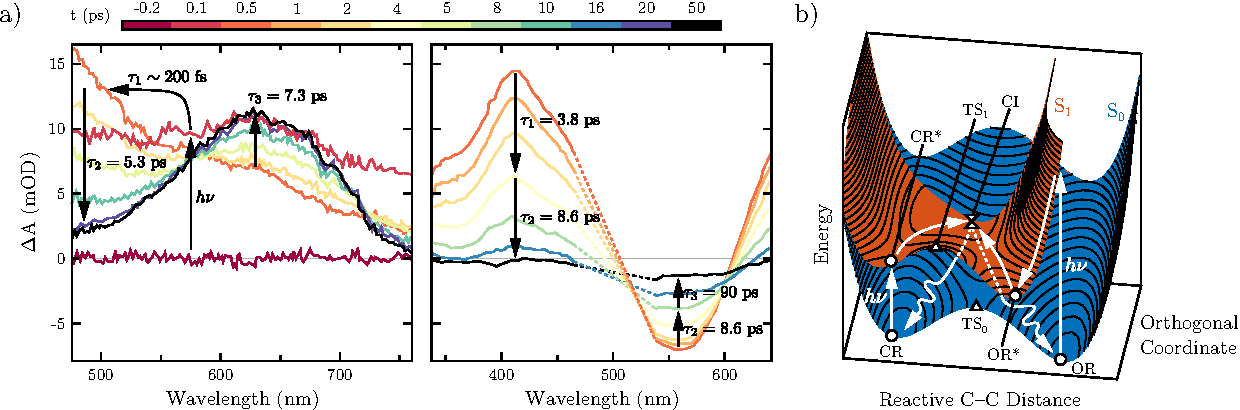
\includegraphics[width = \textwidth]{Figures/fig_DAE_PFC_TA.pdf}
  \caption[Ultrafast reaction dynamics of photochromism.]{
    Ultrafast reaction dynamics of photochromism in PFC:
    (a) transient absorption measurements of the ring-closing (left)
    and ring-opening (right) reactions;
    (b) schematic representation of the two corresponding reaction pathways
    on the S$_0$, S$_1$ potential energy surfaces of a model DAE similar to PFC.
    Panel~(a) is adapted with permission from Refs.~\cite{Jean-Ruel2011}~(left) and~\cite{Ward2012}~(right),
    and Panel~(b), from Ref.~\cite{Boggio2003}.
  }
  \label{fig: DAE-PFC-TA}
\end{figure}

Similarly, the dynamics of the cycloreversion of PFC (in cyclohexane) has been observed
by Ward et al~\cite{Ward2012}.
The right side of Fig.~\ref{fig: DAE-PFC-TA}a shows their femtosecond TA spectra where
there is excited state absorption (ESA) and ground state bleach (GSB)
centered at $410$ and $560$~nm, respectively.
%
In terms of the energy schematic in Panel~(b), the ESA which decays over $\tau_1 = 3.8$~ps
is assigned to dynamics on the S$_1$ surface as the CR molecule evolves to the same conical intersection.
the spectral component with $\tau_2 = 8.6$~ps is the actual ring-opening reaction as the excited state
decays onto the S$_0$ surface;
the GSB disappears over $\tau_3 = 90$~ps as
almost all the photoexcited molecules cool and return to the S$_0$ CR geometry
due to the low quantum yield of photocycloreversion process in PFC.

Since spectroscopic techniques are only sensitive to structural dynamics
through the associated changes in electronic energy levels,
the focus of the UED work presented herein is to directly observe the atomic motions involved in
the photocyclization of single-crystal PFC and
provide a complementary description of the reaction dynamics.

\section{Methods}
\label{sec: UED-DAE-methods}

\begin{figure}[ht!]
  \centering
  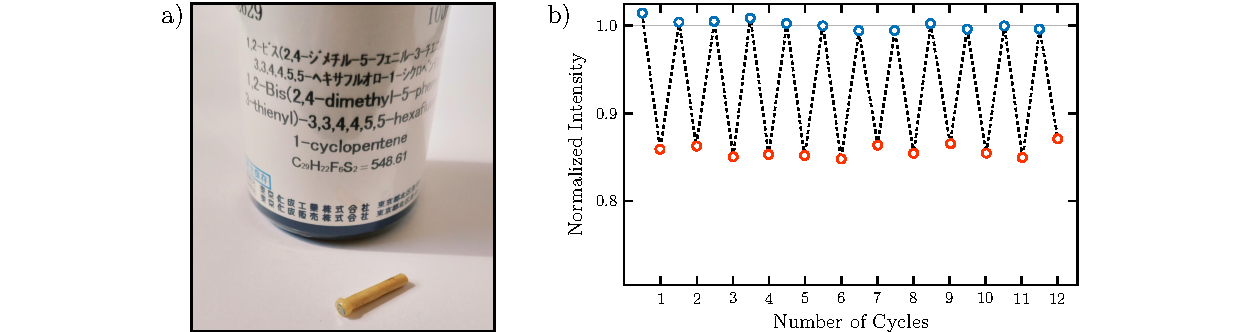
\includegraphics[width = \textwidth]{Figures/fig_DAE_PFC_photo.pdf}
  \caption[Sample preparation and qualification under the pump-probe-HeNe scheme.]{
    (a) Photo of a PFC crystal ready for ultramicrotomy.
    (b) Normalized intensity of the $(5 1 \overline{6})$ diffraction spot
    before (blue) and after (ref) the pump laser pulse for the first 12
    photocyclization--photocycloreversion cycles, showing the reversible transformation
    of single-crystal PFC between its two conformations under the pump-probe-HeNe scheme.
    Panel~(b) is adapted with permission from Ref.~\cite{Jean-Ruel2013}.
  }
  \label{fig: DAE-PFC-Photo}
\end{figure}

% Sample preparation
PFC can be readily synthesized from base reactants using the procedure of Irie et al~\cite{Irie1995}.
Here, it is purchased in powder form from a commercial supplier (Tokyo Chemical Industrial Co.)
and dissolved in hexane at $5$~g/L.
Colourless crystals are grown in the dark by slow solvent evaporation from a flat bottom beaker
and the largest ones (ca.~$500$~$\unslant\mu$m $\times$ 500~$\unslant\mu$m $\times$ 100~$\unslant\mu$m)
are selected for sample preparation.

As in the case of (EDO-TTF)\textsubscript{2}X in Sec.~\ref{sec: UED-EDOPF6}, the chosen crystal
is glued to epoxy resin (Fig.~\ref{fig: DAE-PFC-Photo}a) and cleaved into slices $100$--$150$~nm thick by ultramicrotomy.
These thin single-crystal slices are then mounted on TEM copper mesh grids
with lacy formvar support membranes. To obtain samples with different crystal orientations,
the crystals are cleaved along different planes.

% UED and laser conditions
The UED measurements are conducted in the same experimental setup as in Sec.~\ref{sec: UED-EDOPF6}
with some PFC-specific modifications.
%
To excite the PFC sample near the optimal wavelength for photocyclization,
the pump beam is made by splitting the $267$-nm output of the THG setup before it is
used to generate the probe electron pulses; the fluence and spot size are set to $0.35$~mJ/cm$^2$
and $600$~$\unslant\mu$m at the sample position and the pulses are stretched to ca.~$300$~fs in an effort
to minimize the laser peak power and thus avoid artifacts due to multiphoton ionization.
%
The probe electron pulses are $70$-fC (ca.~$4.4 \times 10^5$~e$^{-}$) bunches
with a spot size of $400$~$\unslant\mu$m FWHM that is centered on the pump spot.
%
Since the closed-ring state of PFC is stable, simply allowing any time between pump-probe events
for thermal relaxation is not feasible to ensure an open-ring sample volume before each measurement.
Instead, a third laser pulse --- $633$~nm, $2$~mW, $100$~ms --- from a helium-neon (HeNe) laser illuminates
the sample $2$~ms after the pump pulse and triggers complete cycloreversion over
a spot size of $700$~$\unslant\mu$m.
%
Thus, the repetition rate of the measurements is necessarily reduced to a paltry $0.1$~Hz,
much slower than that of usual UED experiments.
%
Fig.~\ref{fig: DAE-PFC-Photo}b shows the normalized intensity of a diffraction spot sensitive to
the ring-closing reaction before (blue) and after (red) the pump pulse
for the first dozen (and 400 in the inset) pump-probe-HeNe cycles;
the steadiness of the signal confirms the reversibility of the photoinduced structural dynamics in PFC
under this pump--probe--HeNe scheme.

\begin{figure}[ht!]
  \centering
  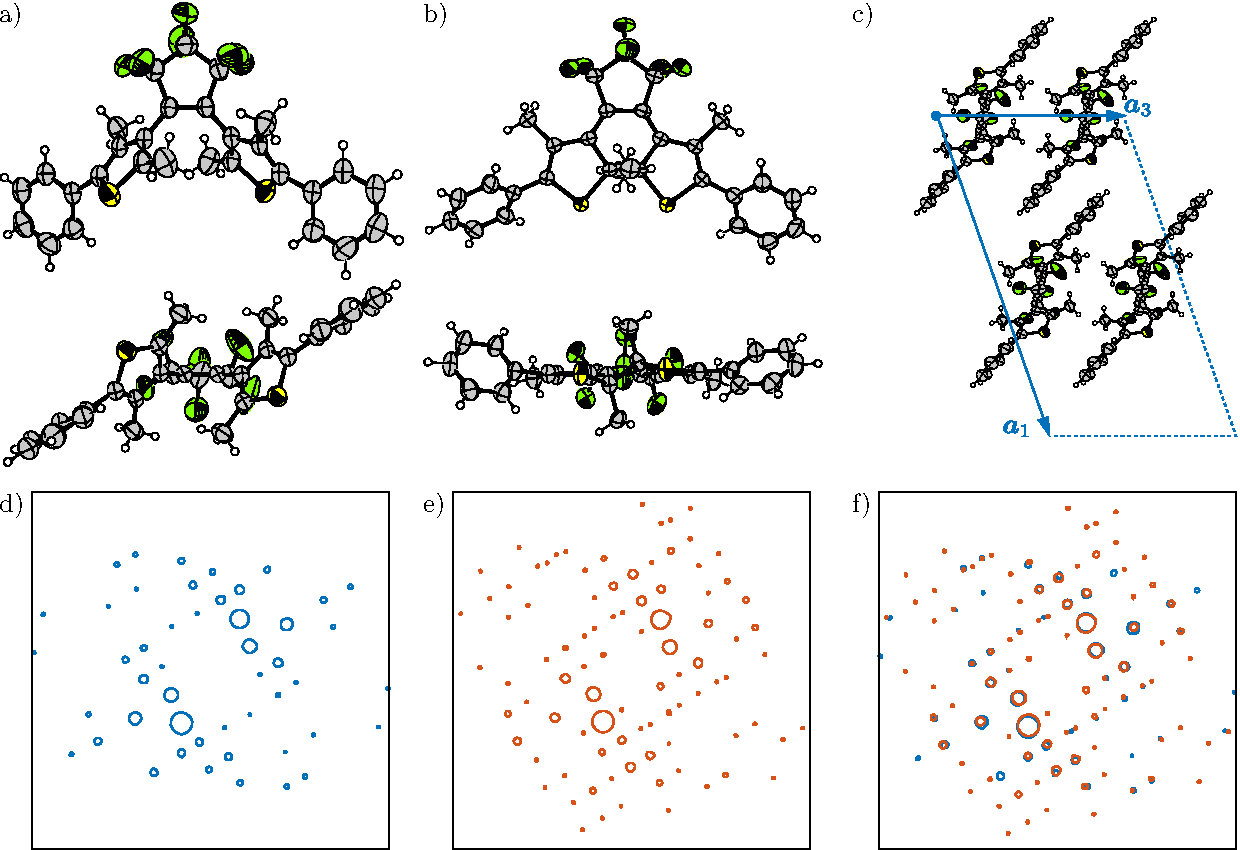
\includegraphics[width = \textwidth]{Figures/fig_DAE_PFC_structure.pdf}
  \caption[Crystal structure of PFC and orientation determination.]{
    ORTEP~representations of the molecular structure of PFC
    in its (a) open-ring and (b) closed-ring conformation,
    and (c) crystal packing in the $(010)$~plane.
    Scatter plots of the (d) experimentally measured and (e) simulated
    diffraction data for a sample with orientation $[ 0.45, 0.19, 0.87]$ are shown
    and (f) overlain for comparison;
    the size of the markers scales with the intensity of the diffraction spots.
    Panels~(a)--(c) and (d)--(f) are adapted with permission from Refs.~\cite{Irie2001}
    and~\cite{Jean-Ruel2013} respectively.
  }
  \label{fig: DAE-PFC-structure}
\end{figure}

To index and interpret the measured UED signals,
the crystal orientation of the samples relative to the incident electron direction needs to be determined.
Here, a simulation-based refinement scheme
--- described in more detail in Sec.~\ref{sec: UED-data-analysis-1} --- is used.
%
The crystal structures of the OR and CR conformers of PFC are shown
in the top three panels of Fig.~\ref{fig: DAE-PFC-structure} from Irie et al~\cite{Irie2001}.
Starting from this information, the simulated intensity and position of diffraction spots
are calculated and matched to the observed values
by maximizing the goodness-of-fit which is the Pearson correlation coefficient $P_\mathrm{sim, exp}$
as in Fig.~\ref{fig: UED-orientation}a.

In the bottom three panels of Fig.~\ref{fig: DAE-PFC-structure},
the experimentally measured and simulated diffraction spots
are compared to show the effectiveness of this refinement scheme.
%
The result is a crystal orientation~$k_\mathrm{inc} = [ u_1, u_2, u_3]$ for each measured PFC sample
with R-factors between $0.23$ and $0.34$.
%
Using these values, Eq.~\eqref{eq: nexc}, and the intensity of 22 reliable diffraction spots,
the excitation fraction $\eta_\mathrm{exc}$ is estimated to be $2.9$~\%,
as expected from the low laser fluence of the pump beam.

To make the molecular movie of PFC, a model of the structural dynamics is needed.
Previously, as in Eq.~\eqref{eq: linear-model},
the atoms are constrained to move linearly between their known ground- and excited-state
positions.
In this case, it is found by inspection that the OR~conformation
can be transformed to the CR~one using only four motions: three rotations
and a rotation plus torsion (see Fig.~\ref{fig: DAE-PFC-model})
%
Then, the measured diffraction intensities can be refined against
those evaluated from this four-parameter model to obtain
a molecular structure of PFC at each probed time point
using the methods described in Sec.~\ref{sec: UED-data-analysis-3}.

\begin{figure}[t!]
  \centering
  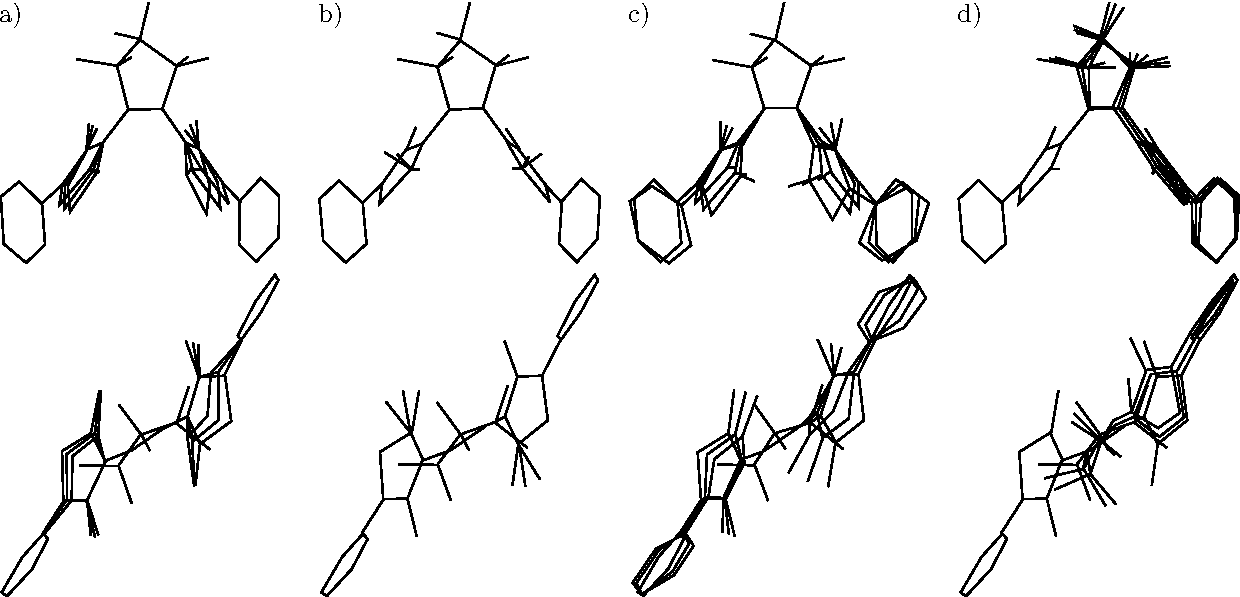
\includegraphics[width = \textwidth]{Figures/fig_DAE_PFC_model.pdf}
  \caption[Four-motion structure model of PFC ring closure.]{
    Front and top skeleton view of the four motions which transform the PFC molecule
    from its OR ($\xi = 0$) to CR ($\xi = 1$) conformation in two steps of $\Delta \xi = 0.5$.
    Adapted with permission from Ref.~\cite{Jean-Ruel2013}.
  }
  \label{fig: DAE-PFC-model}
\end{figure}

% Computational methods
In support of the UED molecular movie, an ab initio model of the ring closing reaction
in the single-crystal state is implemented in the subtractive QM/QM paradigm,
a hybrid computational scheme that offers reasonable accuracy in large molecular systems.
%
Briefly, the set of all atoms $\mathbb{S}$ is partitioned into an inner subset $\mathbb{I}$
and an outer subset $\mathbb{O}$ consisting respectively of the few atoms of the reaction centre
and the many others that are mostly spectators;
different levels of quantum mechanical approximation can then be applied,
with the highest and computationally most expensive level one $\mathbb{I}$ and the lowest on $\mathbb{O}$,
and the total QM/QM energy of the system is thus given by
%
\begin{equation}
  \begin{aligned}
    E_\mathrm{QM/QM}(\mathbb{S}) & = E_\mathrm{LQM}(\mathbb{S})
      + E_\mathrm{HQM}(\mathbb{I} \cup \mathbb{L}) - E_\mathrm{LQM}(\mathbb{I} \cup \mathbb{L})
  \end{aligned}
  \label{eqn: QMQM}
\end{equation}
%
where $\mathrm{HQM}$ and $\mathrm{LQM}$ are applicable high- and low-level QM methods and
$\mathbb{L}$ is the set of `linkers,' extra hydrogen atoms added to cap any dangling covalent bond
in the boundary between $\mathbb{I}$ and $\mathbb{O}$~\cite{Senn2006, Vreven2006, Kochman2013}.
%
Here, the UED sample is modeled as a bulk lattice where only one of the four PFC molecules
in the unit cell is photoreactive.
In the QM/QM scheme of this work, $\mathbb{S}$ is the set of all the atoms in a single unit cell
and $\mathbb{I}$ consists of the 1,2-bis(2,4-dimethyl-3-thienyl)pentene moiety
of one of the PFC molecules (see Fig.~\ref{fig: DAE-PFC-QMQMmodel}).
%
$E_\mathrm{LQM}(\mathbb{S})$ is calculated on the level of density functional theory~(DFT)
using a plane wave basis set%
\footnote{The plane wave cut-off is set at 400~eV;
the electronic Brillouin zone is sampled at the $(0 \frac{1}{4} 0)$ $k$-point only;
the default ultrasoft pseudopotentials in \textsc{CASTEP} are used;
energies and forces are corrected for dispersion interactions as in Ref.~\cite{Grimme2006}.}
and the Perdew-Burke-Ernzerhof~(PBE) exchange-correlation functional
as implemented in \textsc{CASTEP}~5.0;
%
$E_\mathrm{LQM}(\mathbb{I} \cup \mathbb{L})$ is similarly evaluated but
using the localized Gaussian-type 3-21G(d) orbital basis.
%
Finally, $E_\mathrm{HQM}(\mathbb{I} \cup \mathbb{L})$ is calculated at the level of
complete-active-space self-consistent field~(CASSCF) theory%
\footnote{An active space consisting of 10 canonical $\pi$- and $\pi^*$-type orbitals
is used.} as implemented in \textsc{Gaussian}~09 using the localized 3-21G basis set.

\begin{figure}[ht!]
  \centering
  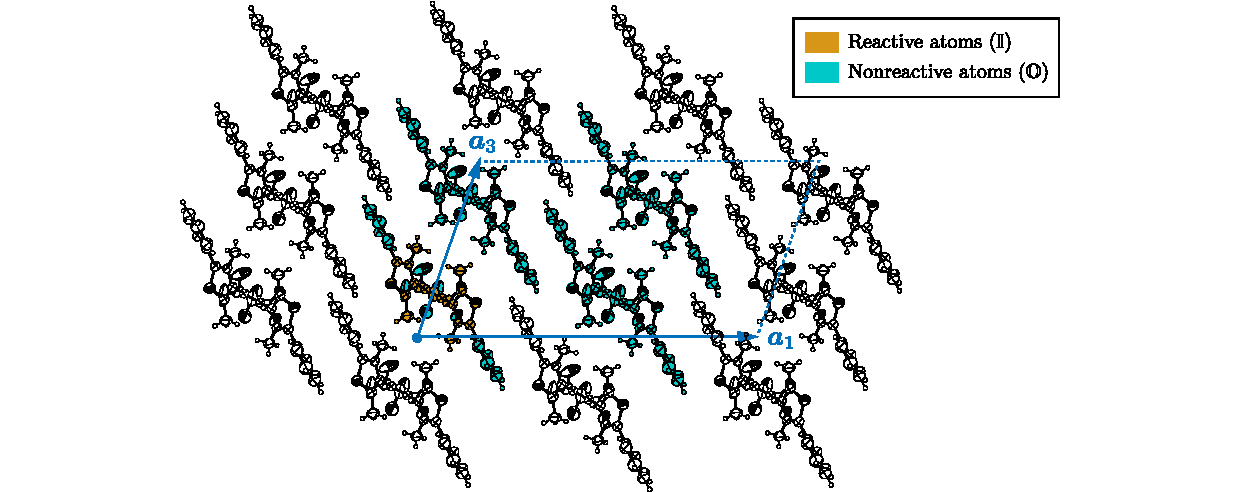
\includegraphics[width = \textwidth]{Figures/fig_DAE_PFC_QMQMmodel.pdf}
  \caption[Partitioning of PFC unit for QM/QM~calculations.]{
    Partitioning of the atoms of the PFC~unit cell into two subsets, $\mathbb{I}$ and $\mathbb{O}$,
    for hybrid QM/QM calculations.
    Adapted with permission from Ref.~\cite{Irie2001, Jean-Ruel2013}.
  }
  \label{fig: DAE-PFC-QMQMmodel}
\end{figure}


\section{Experimental Results and Discussion}
\label{sec: UED-DAE-results}

% UED patterns
In Fig.~\ref{fig: DAE-PFC-UED}, time-resolved electron diffraction data
of single-crystal PFC are shown in three different crystal orientations.
From Panels~(a)--(c), the patterns are well ordered to high diffraction orders and
many spots can be clearly observed.
%
To evaluate the sensitivity of the UED setup to the ring-closing reaction,
pump-probe UED images are taken at a time delay corresponding to $t_\infty$
and compared to simulated ones, calculated using Eq.~\eqref{eq: diff-int}
and the known XRD structures of the open- and closed-ring molecules from Ref.~\cite{Irie2001}.
%
These $t_\infty$ difference images are shown in Panels~(d)--(f) and
it can be observed that a large number of diffraction spots exhibit
significant and divergent changes in intensity, indicative of
atomic displacement within the unit cell.
%
The close match between these changes with the simulated ones in Panels~(g)--(i)
demonstrates that UED can probe the relevant structural dynamics of PFC.
%
\begin{figure}[ht!]
  \centering
  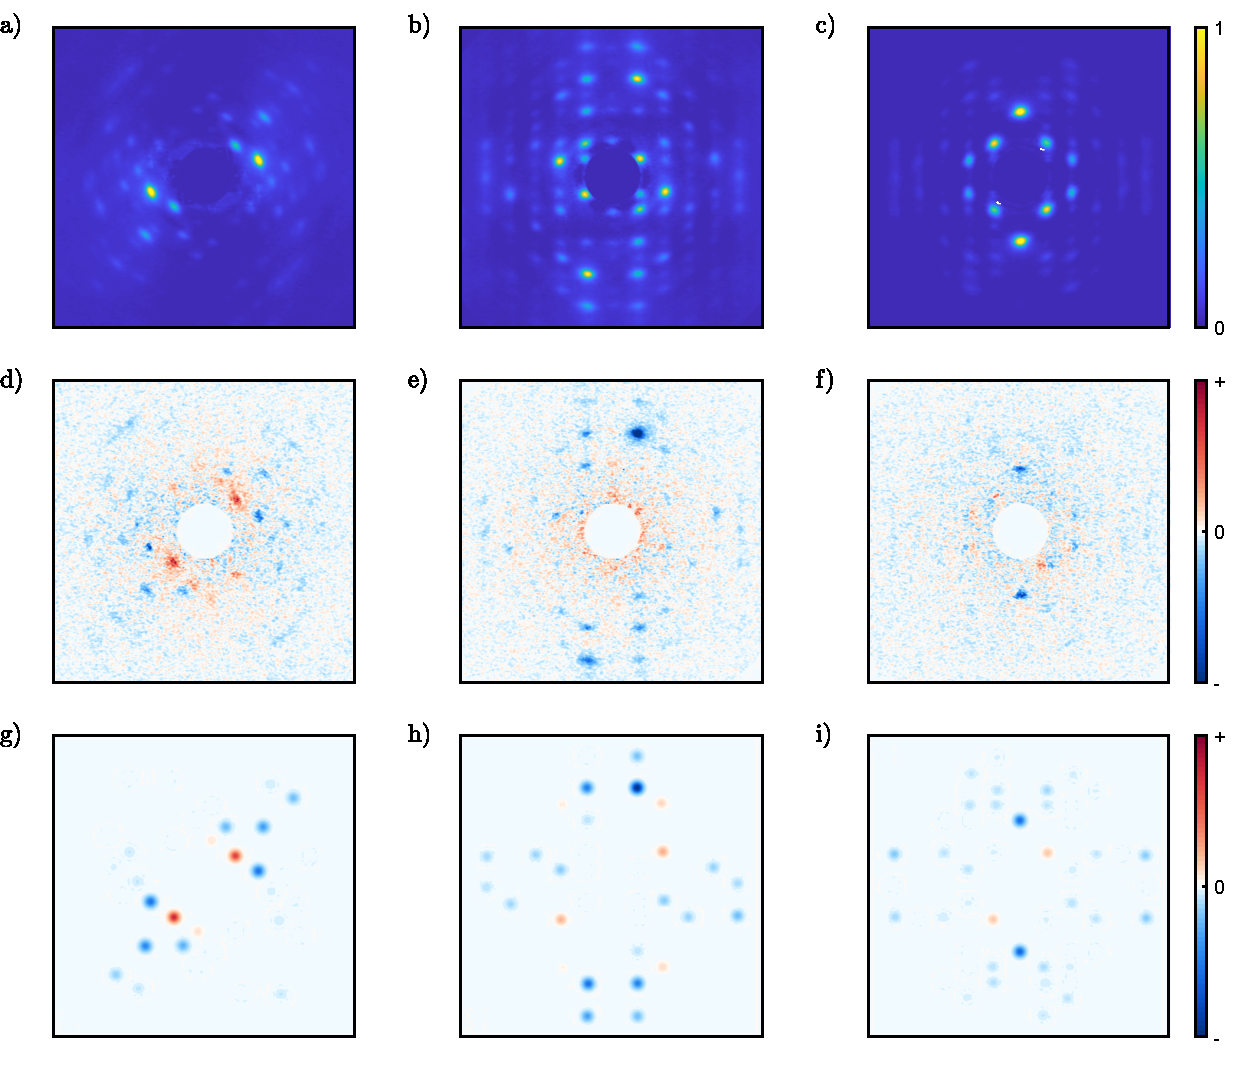
\includegraphics[width = \textwidth]{Figures/fig_DAE_PFC_UED_.pdf}
  \caption[Time-resolved electron diffraction patterns of PFC.]{
    Time-resolved electron diffraction data of PFC samples
    with different crystal orientations:
    (a) $[ 0.45, 0.19, 0.87]$; (b) $[ -0.77, 0.17, -0.62]$; (c) $[ 0.87, -0.02, 0.49]$.
    Row-wise, Panels~(a)--(c) show the static UED patterns;
    (d)--(f), the pump-probe difference intensities at $t_\infty$;
    (g)--(i), the simulated difference intensities assuming an excitation fraction of $2.9$~\%
    and using the known XRD structures of the open- and closed-ring molecules.
    Adapted with permission from Ref.~\cite{Jean-Ruel2013}.
  }
  \label{fig: DAE-PFC-UED}
\end{figure}

% Time traces
Fig.~\ref{fig: DAE-PFC-UEDtraces} shows the temporal evolution in intensity of four select
diffraction spots, chosen because they are representative of all the changes observed
in the UED dataset of PFC.
%
\begin{figure}[ht!]
  \centering
  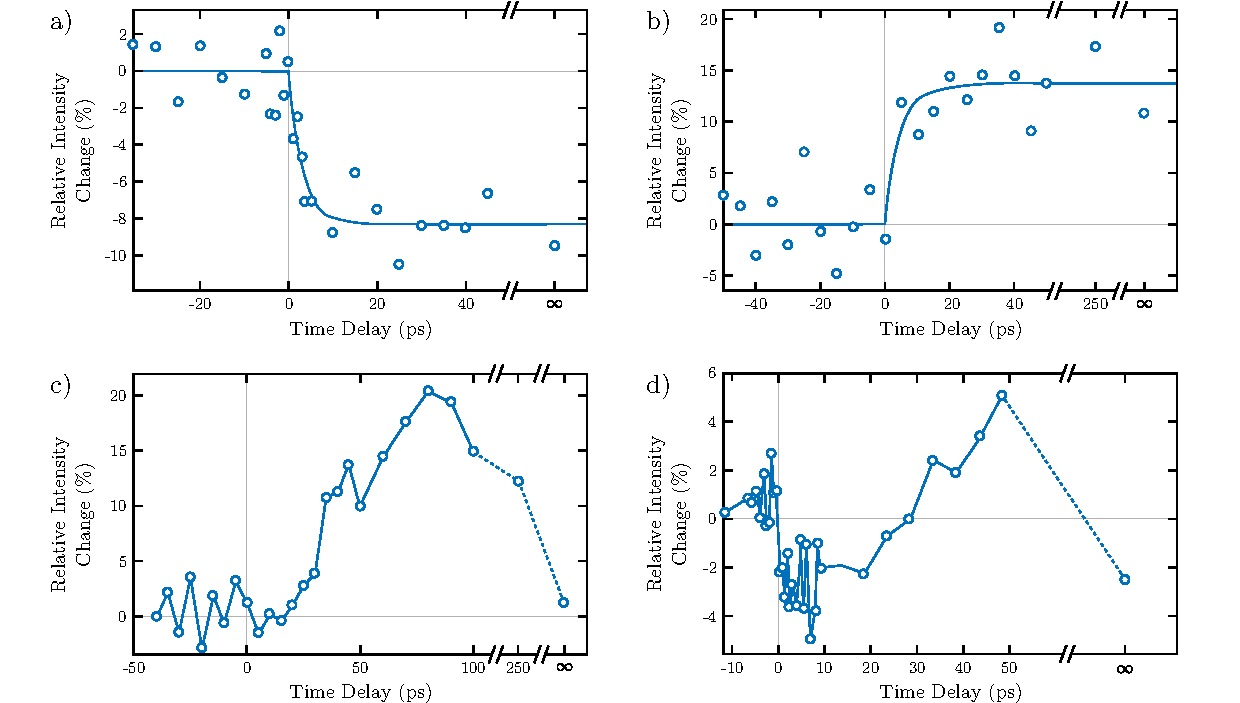
\includegraphics[width = \textwidth]{Figures/fig_DAE_PFC_UEDtraces.pdf}
  \caption[Select UED time traces of single-crystal PFC.]{
    Select UED time traces of single-crystal PFC showcasing
    the different type of time-dependent intensity changes
    in the measured diffraction patterns:
    (a) $(5 1 \overline{6})$;
    (b) $(5 \overline{1} \overline{2})$;
    (c) $(2 0 \overline{2})$;
    (d) $(2 0 \overline{4})$.
    Adapted with permission from Ref.~\cite{Jean-Ruel2013}.
  }
  \label{fig: DAE-PFC-UEDtraces}
\end{figure}

The UED signals in Panels~(a) and (b) are typical to many diffraction spots:
an ultrafast change that develops over a few picoseconds and stays until $t_\infty$.
Since the $t_\infty$ intensity difference corresponds to the closed-ring structure,
they are directly attributed to the structural dynamics associated with
the ring-closing reaction.
Furthermore, monoexponential fit of these two time traces yield
two different time constants: $\tau_1 = (3 \pm 1)$~ps and $\tau_2 = (5 \pm 3)$~ps respectively.
These values agrees with the results of previously reported TA measurements~\cite{Jean-Ruel2011},
where a time constant of $5.3$~ps was found for the orthogonal evolution of
excited state on the S$_2$ potential energy surface from the excited open-ring intermediate (OR$^*$)
to the closed-ring (OR) structure (see Fig.~\ref{fig: DAE-PFC-TA}b).

Fig.~\ref{fig: DAE-PFC-UEDtraces}c shows another type of UED signal that is observed
for a number of diffraction spots; it consists of a very slow $80$-ps change of large amplitude
that vanishes between $t = +100$~ps and $t_\infty$.
This transient behaviour does not reflect the thermally irreversible structural change
associated with photocyclization.
Instead, it is indicative of strain waves generated by the mechanical stress of
some PFC molecules contracting volumetrically as they are photoexcited and undergo ring closure.
From Ref.~\cite{Irie2001}, a PFC molecule flattens and shrinks during the OR$\rightarrow$CR transformation,
with its width%
\footnote{As measured by the distance between the methyl groups ortho to the reactive carbon atoms.}
decreasing by ca.~$20$~\%.
Similar strain signals are observed in the late-time UED data of (EDO-TTF)\textsubscript{2}X
(see the left side of Fig.~\ref{fig: EDO-TRresults}b).
Conveniently, since these intensity changes are few, easily identified as signal modulations,
and well separated in time, they do not prevent the monitoring of the photocyclization process by UED.
Indeed, the Pearson correlation coefficient between
the experimental $\Delta I/I_\mathrm{off}$ averaged over $t = +10$ and $+50$~ps and
the simulated ones is $0.92$ when only strain-free diffraction spots are considered.

Finally, Fig.~\ref{fig: DAE-PFC-UEDtraces}d presents a UED signal
that clearly appears within a picosecond and is followed by a slow transient feature
caused by the crystal strain.
The observation of this ultrafast signal is a key result of the present work
since its time scale is consistent with that of the evolution on the S$_2$ potential energy surface
prior to ring closure ($\tau_1$ in the left side of Fig.~\ref{fig: DAE-PFC-TA}a),
from the initial open-ring Franck-Condon state to the open-ring intermediate state
(OR$^*$ in Fig.~\ref{fig: DAE-PFC-TA}b).
Thus, the existence of an intermediate PFC structure, forming in these times and
clearly distinct from the closed-ring one, is confirmed.

% Model results
% Figure: 0 ps, +10 ps structures, histogram
To reconstruct the real-space molecular movie of PFC as it undergoes photocyclization,
the four-motion model set up in Fig.~\ref{fig: DAE-PFC-model} is employed,
with a focus on the structure of the intermediate state that forms soon after photoexcitation.
%
As prescribed in Sec.~\ref{sec: UED-data-analysis-3},
the four components of the reaction coordinate $\boldsymbol{\xi} = (\xi_1, \xi_2, \xi_3, \xi_4)$
are independently varied from $-0.5$ to $1.5$ to generate a large pool of candidates,
where the coordinates $\boldsymbol{\xi} = (0, 0, 0, 0)$ and $(1, 1, 1, 1)$ represent
the ground OR and CR structures respectively (see Panels~(a) and (b) of Fig.~\ref{fig: DAE-PFC-results}).
%
The structure factors of each generated structure, $F_\mathrm{sim}(\boldsymbol{\xi}), \boldsymbol{q}_j$,
is then simulated under the kinematical approximation and compared to the experimentally measured one,
$F_\mathrm{on, exp}(t, \boldsymbol{q}_j)$, using the Pearson correlation coefficient,
$P_\mathrm{sim, exp}(\boldsymbol{\xi}, t)$, as the GoF.
%
Given the limited~SNR of the experimental data, the analysis uses only
the $18$~brightest strain-free diffraction spots and the optimal reaction coordinate
for a given time point, $\boldsymbol{\xi}_\mathrm{opt}(t)$,
is defined as the average of the subset of coordinates
which generates the top $1$~\% best-matching structures.

\begin{figure}[t!]
  \centering
  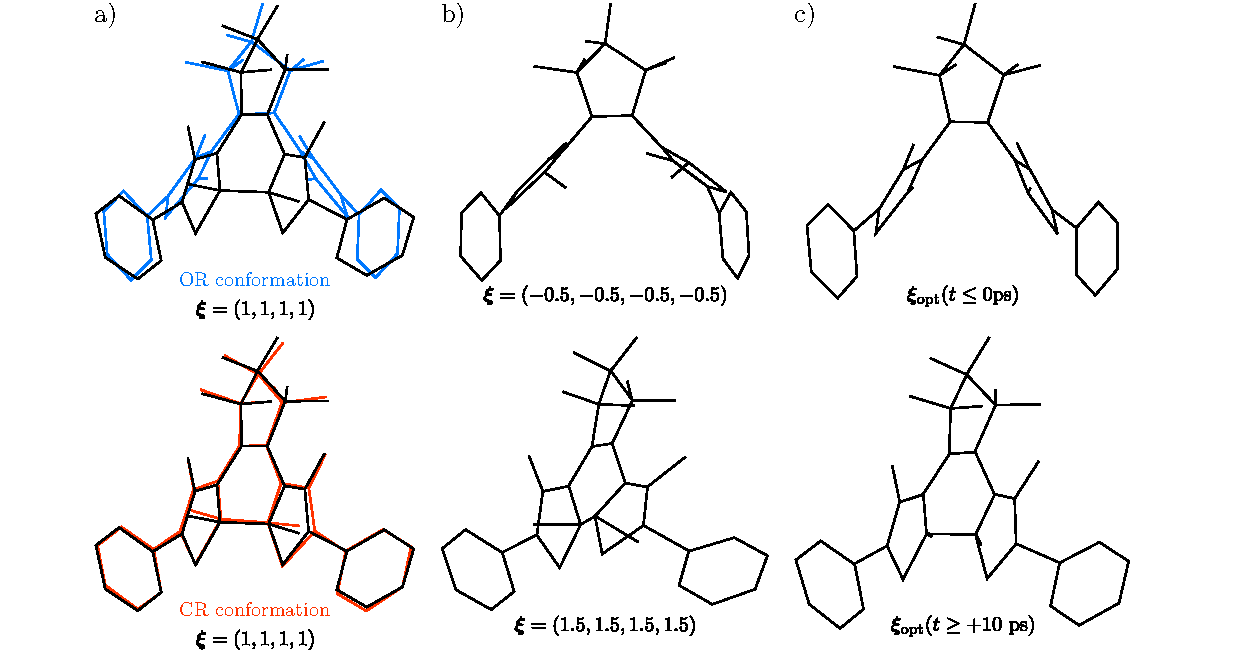
\includegraphics[width = \textwidth]{Figures/fig_DAE_PFC_results.pdf}
  \caption[Structural dynamics of PFC in the four-motion model.]{
    Structural dynamics of PFC in the four-motion model:
    comparing (a) the $(1, 1, 1, 1)$ structure with those of
    the ground conformations after geometry optimization;
    (b) the lower and upper bounds of the searched coordinate space;
    (c) the optimal structures that best fit the pump-off ($t \leq 0$~ps)
    and late-time ($t \geq 10$~ps) data.
    Adapted with permission from Ref.~\cite{Jean-Ruel2013}.
  }
  \label{fig: DAE-PFC-results}
\end{figure}

In Fig.~\ref{fig: DAE-PFC-results}c, the model PFC structures
generated by $\boldsymbol{\xi}$ optimized for the pump-off ($t \leq 0$~ps)
and late-time ($t \geq 10$~ps) diffraction data are shown.
By inspection, both are consistent with the known structures of
the ground OR and CR conformers.
%
The positions of the two methyl groups ortho to the reactive carbon atoms
have not converged to their expected CR values, likely due to
weak contribution to the diffraction intensities in the crystal orientations sampled here.

A key point of interest in the photocyclization process of PFC is
the structural dynamics that occur at early time,
before the actual ring closure itself.
%
Here, inspection of $\boldsymbol{\xi}_\mathrm{opt}(t)$ for $t$ from $+0.5$ to $+3.0$~ps
(see Fig.~\ref{fig: DAE-PFC-results-QMQM}a) suggests that
the dominant atomic motion resolved in the UED data is
a full rotation of the thiophene moieties combined with
a partial rotation of the perfluorocyclopentene ring.
%
This conformation is distinct from those of the ground states (OR and CR);
it is tentatively assigned to the open-ring excited state (OR$^*$ in Fig.~\ref{fig: DAE-PFC-TA}b)
proposed by the theoretical work of Boggio-Pasqua et~al
for a free PFC molecule~\cite{Boggio2003}.

To validate the assignment of the early-time UED intermediate to
the OR$^*$ state, ab initio calculations are performed,
extending the Boggio-Pasqua work~\cite{Boggio2003} to the single-crystal phase.
%
As described in Sec.~\ref{sec: UED-DAE-methods} and shown in Fig.~\ref{fig: DAE-PFC-QMQMmodel},
the reaction centre of the photoexcited molecule is described at the CASSCF level of theory
while the rest of the molecule and unit cell is treated at the lower DFT level.
The result is a reaction intermediate embedded in a crystal lattice of ground-state molecules,
all fully optimized.
%
It is found that this structure is in the OR conformation with a shortened distance of $2.19$~\AA{}
between the two reactive carbon atoms, halfway between the corresponding values of the OR and CR ground states
($3.71$~\AA{} and $2.204$~\AA{} respectively) and fully consistent with
the structure of the intermediate state OR$^*$ in Ref.~\cite{Boggio2003}.
%
Little structural distortion occurs amongst the nonreactive OR molecules of the bulk crystal.

In Fig.~\ref{fig: DAE-PFC-results-QMQM}b,
the optimized geometries of the OR ground state and the reaction intermediate are compared.
Here, it can be seen that the thiophene rings become significantly rotated
while the phenyl and perfluorocyclopentene rings are relatively unchanged.
Indeed, these structural changes are qualitatively in agreement with
those that captured experimentally by UED (Fig.~\ref{fig: DAE-PFC-results-QMQM}a).

\begin{figure}[t!]
  \centering
  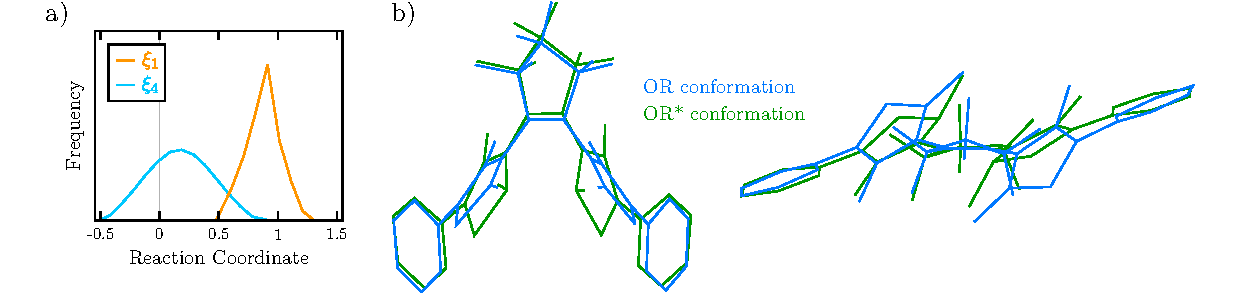
\includegraphics[width = \textwidth]{Figures/fig_DAE_PFC_resultsQMQM.pdf}
  \caption[Molecular Structure of PFC photocyclization intermediate.]{
    Molecular Structure of PFC photocyclization intermediate.
    (a) Frequency distribution of the dominant atomic motions
    amongst the top $1$~\% best-matching structures for $t$ from $+0.5$ to $+3.0$~ps
    as resolved by UED.
    (b) Front and top skeleton view of the theoretical
    ground- (blue) and excited-state (green) open-ring structures,
    as determined by the hybrid QM/QM model.
    Adapted with permission from Ref.~\cite{Jean-Ruel2013}.
  }
  \label{fig: DAE-PFC-results-QMQM}
\end{figure}

Overall, the results of the present work --- experimental and computational ---
strongly support the reaction mechanism suggested previously for describing
the photocyclization of PFC~\cite{Boggio2003, Jean-Ruel2011}.
Following photoexcitation and internal conversion from higher-lying states
to the S$_1$ potential energy surface, the OR molecule quickly relaxes from
the Franck-Condon geometry to OR$^*$, an OR minimum on the S$_1$
along the `reactive C--C' reaction coordinate.
%
Analysis of the measured changes in diffraction intensity confirm that this relaxation pathway
involves significant atomic motions which occur on the subpicosecond time scale;
details of the intermediate structure are provided by
the results of the QM/QM-based computational model.
%
Later, the large amount of kinetic energy released during the relaxation is redistributed amongst
various vibrational modes of the molecule.
Some of these become motions orthogonal to the main reaction coordinate that drive
the system to a conical intersection (CI in Fig.~\ref{fig: DAE-PFC-TA}b)
where it decays radiationlessly back to the S$_0$ surface and completes the ring closure.
%
This last convergence to the CR structure is also unambiguously witnessed with UED
and therein confirmed to occur with a time constant of ca.~$ 5$~ps.

Note that, in the quantum chemical calculations,
the photoexcited molecule is not entirely treated at the CASSCF level;
the fluorine atoms and those of the pendant phenyl groups are relegated
to the outer subset $\mathbb{O}$ to reduce the computation time to
a manageable duration.
This approximation is a weakness of the model which may be improved later.
%
Furthermore, it is not clear from the calculations whether the intermediate structure
captured in UED is necessarily the OR$^*$ conformation
or a mixture of nearby states, possibly involving other conical intersections.
Further theoretical investigation would be required to resolve this question.


\section{Summary and Conclusions}

In this work, UED measurements are performed with subpicosecond temporal resolution
to investigate the structural dynamics involved in the photocyclization of
single-crystal PFC, a photochromic diarylethene derivative.
%
The fatigue resistance and thermal irreversibility of this molecular system
is exploited to directly resolve the formation of a reaction intermediate
and subsequent convergence to the closed-ring photoproduct.

A key result is the observation that a few atomic motions can fully transform
the open-ring molecule to the closed-ring one.
Using this insight, a low-dimensional structure model of PFC is constructed
to refine the atomic positions of the molecule from the UED images
for every sampled time point.
%
Note that such dramatic reduction in dimensionality in barrier crossing regions
should be a general observation in complex organic systems;
indeed, this is what makes chemistry a transferable subject.
%
It is likely that this reduction is enabled by coupling between
low-frequency spatially extended modes and high-frequency localized modes
of the molecule.
%
Understanding the exact nature of this coupling is a central issue in chemistry
since it pertains to how far-from-equilibrium fluctuations are involved in
chemical processes.
%
Since the specific atomic motions cannot be inferred from static molecular structures alone,
the present work thus demonstrates the use of UED to determine these key modes.
